\section{Working Resources Area}
The Working Resource Area encompass all the AllSpark's business processes that characterize its right lifecycle and functionalities releated to the working environment. Each business process aims to satisfy some specific objective needed by correctness and the efficiency of processes in other areas, but that are not required in advance for the productivity roles the Company wants to achieve. The employees involved in the business processes are potentially of all kind foreseen in the Working Structure presented in figure \ref{2img:working}.

A particular observation is reserved to the responsibility role of this Area. Since each area has a responsible the discussion about it is relavant, but not so simple to define a unique responsible except for the CEO; generally is defined an Area Manager that leads all the business processes, but pratically is more efficient that each process is assigned to the most similar manager.

The business process Systems management has not been modeled since is very general and most of its processes are not really interesting.

\subsection{Updating Management}
This Updating Management business process is derived by the macro business process ``Systems Management'' that provides, as the name suggests, the service of ``up to date'' systems meaning softwares, both products and tools, and hardwares in order to minimize the presence of bugs, improve the efficiency and acquire new features.

The main responsible of this business process is the System Manager who has the very important role of manage all the tasks reducing the possible side effects. For certain task the System Manager is not required to be responsible since are not warning activities. The whole process is shown in figure \ref{2img:updating}.

\begin{figure}[ht!]
\begin{centering}
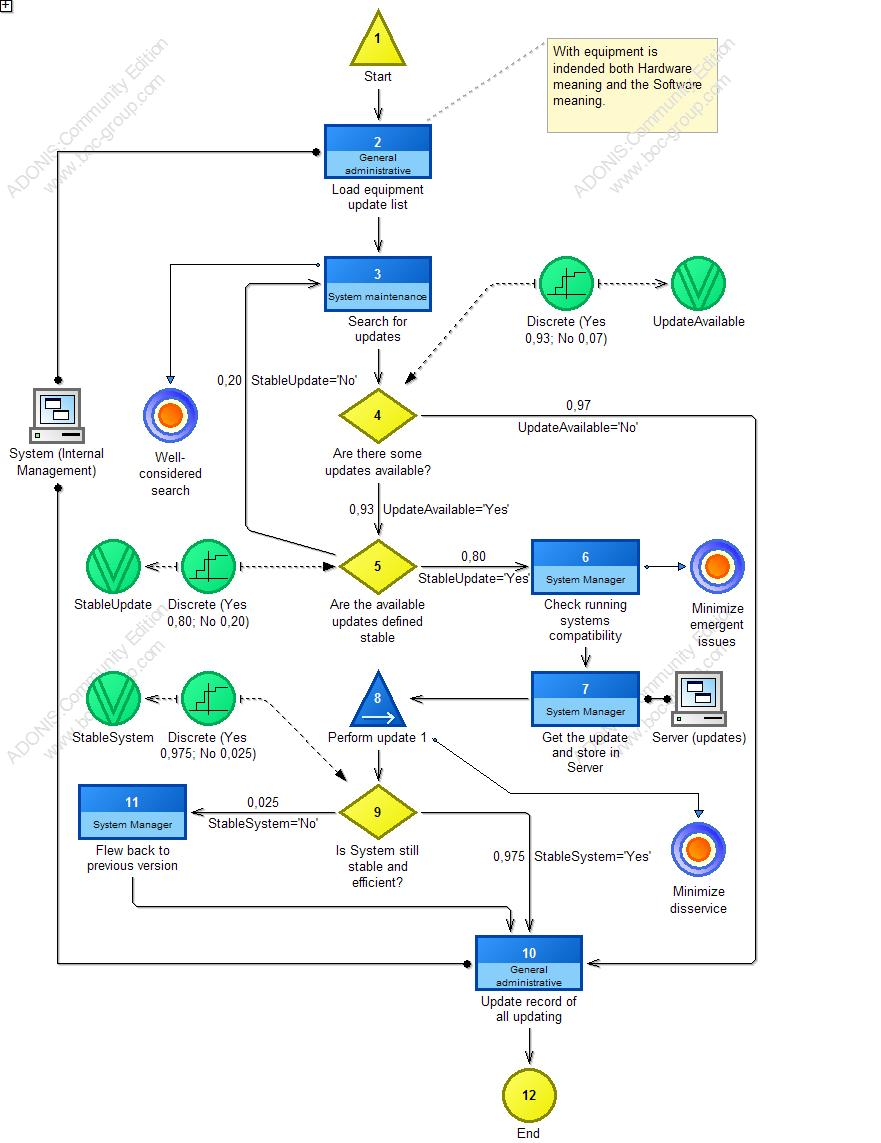
\includegraphics[scale=0.50]{assign2/adonis/imgs/updating.jpg}
\caption{AllSpark Updating Management.}
\label{2img:updating}
\end{centering}
\end{figure}


\subsubsection{Path Analysis}
According to the results of path analysis, an update is expected to succeed with the probability of 73,70\% as foreseen. The whole process is quite cheaper and the time is considered with nothing going badly. The following report returns the complete information about it.

\begin{alltt}
Probability:   73,7000\%
Execution time:  00:000:01:21:00
Waiting time:  00:000:00:02:00
Resting time:  00:000:00:12:00
Transport time:  00:000:00:10:00
Cycle time:  00:000:01:45:00
Costs:  1,980000

Updating Management 0.3 (Business process model)
========================================
Process start: Start
Activity: Load equipment update list
Activity: Search for updates
Decision: Are there some updates available? --> UpdateAvailable='Yes'
Decision: Are the available updates defined stable --> StableUpdate='Yes'
Activity: Check running systems compatibility
Activity: Get the update and store in Server
Subprocess: Perform update
Decision: Is System still stable and efficient? --> StableSystem='Yes'
Activity: Update record of all updating
End: End

Updating Management 0.3 (Business process model) --> Perform update 1 (Business process model)
========================================
Process start: Start
Activity: Perform update
End: End
\end{alltt}


\subsubsection{Capacity Analysis}
The capacity analysis for this process shows the interesting activites' report which are strongly dependent by the System Manager which is represented by either Sysadmin or Area Manager distinguishing the cases in which he is the real responsible of the entire AllSpark's system structure.

\begin{landscape}
\begin{table}
\centering
{\tiny
\begin{tabular}{|l|l|l|l|l|l|l|}
Business process&Activity&Performer&Number&Execution time&Cycle time&Costs\\
\hline
Updating Management 0.3&&&&00:000:01:23:33&00:000:01:48:07&5,966800\\
\hline
&Load equipment update list &&1,000000&00:000:00:01:00&&0,200000\\
\hline
&&Secretary &1,000000&00:000:00:01:00&&0,200000\\
\hline
&Update record of all updating &&1,000000&00:000:00:15:00&&0,900000\\
\hline
&&Secretary &1,000000&00:000:00:15:00&&0,900000\\
\hline
&Search for updates &&1,240000&00:000:00:24:48&&0,248000\\
\hline
&&Sysadmin &1,240000&00:000:00:24:48&&0,248000\\
\hline
&Check running systems compatibility &&0,910000&00:000:00:09:06&&0,273000\\
\hline
&&Area Manager &0,910000&00:000:00:09:06&&0,273000\\
\hline
&Flew back to previous version &&0,020000&00:000:00:01:48&&4,000000\\
\hline
&&Area Manager &0,020000&00:000:00:01:48&&4,000000\\
\hline
&Get the update and store in Server &&0,910000&00:000:00:13:39&&0,273000\\
\hline
&&Area Manager &0,910000&00:000:00:13:39&&0,273000\\
\hline
&Perform update &&0,910000&00:000:00:18:12&&0,072800\\
\hline
&&Sysadmin &0,910000&00:000:00:18:12&&0,072800\\
\hline
Total&&&&00:000:01:23:33&&5,966800
\end{tabular}
}
\caption{Capacity analysis for Updating Management.}
\end{table}
\end{landscape}
%

%

\subsection{Security checking}
The ``Security checking'' business process scope is to achieve the best protection through prevention against introuders, external penetration attempts, system's robustness and security, reliability with high load application and stability. To performing all the test, sometime is necessary to require a professional\footnote{In particular penetration test are aimed by AllSpark to certificate its quality.} that has experience in this kind of application and, over all, that is costantly up to date with respect to the always new method to trick the barriers.

Since the test concern both implemented product and the acquired product, the main responsible of all the operation is located on the Project management role which sorround all the aspect of the Company's system. The testing functionalities are followed also by some elements of ``Research \& Development'' organizational unit, represented in figure \ref{2img:working}, in order to furnish detailed parameters and to acquire testing metodologies.

\begin{figure}[ht!]
\begin{centering}
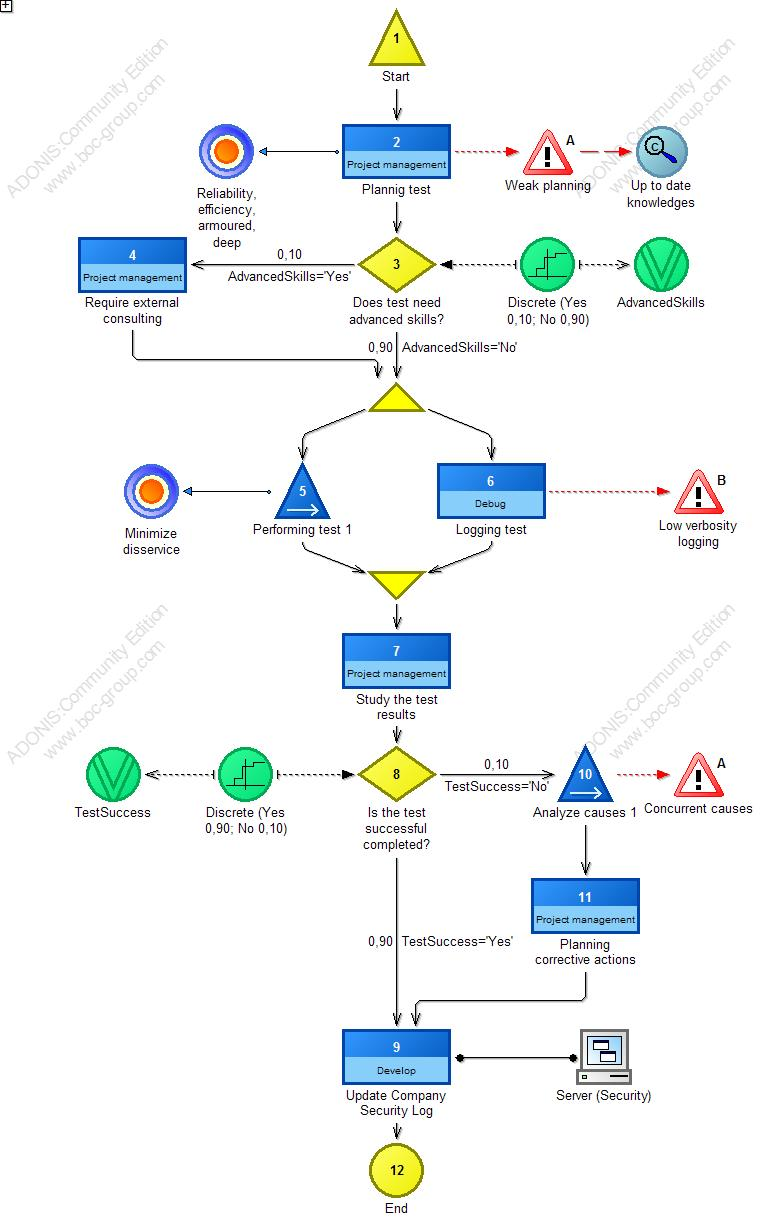
\includegraphics[scale=0.50]{assign2/adonis/imgs/security.jpg}
\caption{AllSpark Security checking.}
\label{2img:security}
\end{centering}
\end{figure}


\subsubsection{Path Analysis}
A path leads with the 80,20\% of probability above the all others resulting by the path analysis. The timing is quite interesting since in about two hours is possible to indicate the characteristics of the Systems. This time excludes eventually a deep penetration test which requires day of work in order to acquire sensitive information to use against the AllSpark.

\begin{alltt}
Probability:   80,2000\%
Execution time:  00:000:02:05:00
Waiting time:  00:000:00:03:00
Resting time:  00:000:00:00:00
Transport time:  00:000:00:05:00
Cycle time:  00:000:02:08:00
Costs:  2,510000

Security Checking 0.1 (Business process model)
========================================
Process start: Start
Activity: Plannig test
Decision: Does test need advanced skills? --> AdvancedSkills='No'
Parallelity: Parallelity-21893
    *
    Activity: Logging test
    *
    Subprocess: Performing test
Merging: Merging-21898
Activity: Study the test results
Decision: Is the test successful completed? --> TestSuccess='Yes'
Activity: Update Company Security Log
End: End

Security Checking 0.1 (Business process model) --> Performing test 1 (Business process model)
========================================
Process start: Start
Activity: Performing test
End: End
\end{alltt}


\subsubsection{Capacity Analysis}
The capacity analysis of this process shows the interesting variation of Execution time from the Cycle time. This element underline the great difference in the concept of real execution versus the concept of the factors that may involve in a determined task as in this case.

\begin{landscape}
\begin{table}
\centering
{\tiny
\begin{tabular}{|l|l|l|l|l|l|l|}
Business process&Activity&Performer&Number&Execution time&Cycle time&Costs\\
\hline
Security Checking 0.1&&&&00:000:02:14:24&00:000:03:24:49&8,014000\\
\hline
&Plannig test &&1,000000&00:000:00:20:00&&1,000000\\
\hline
&&Analyst &1,000000&00:000:00:20:00&&1,000000\\
\hline
&Require external consulting &&0,108000&00:000:00:01:05&&5,400000\\
\hline
&&Analyst &0,108000&00:000:00:01:05&&5,400000\\
\hline
&Logging test &&1,000000&00:000:00:05:00&&0,010000\\
\hline
&&Programmer &1,000000&00:000:00:05:00&&0,010000\\
\hline
&Study the test results &&1,000000&00:000:00:30:00&&0,500000\\
\hline
&&Analyst &1,000000&00:000:00:30:00&&0,500000\\
\hline
&Planning corrective actions &&0,104000&00:000:00:02:05&&0,052000\\
\hline
&&Analyst &0,104000&00:000:00:02:05&&0,052000\\
\hline
&Update Company Security Log &&1,000000&00:000:00:10:00&&0,000000\\
\hline
&&Programmer &1,000000&00:000:00:10:00&&0,000000\\
\hline
&Performing test &&1,000000&00:000:01:00:00&&1,000000\\
\hline
&&Area Manager &1,000000&00:000:01:00:00&&1,000000\\
\hline
&Performing test &&0,104000&00:000:00:06:14&&0,052000\\
\hline
&&Area Manager &0,104000&00:000:00:06:14&&0,052000\\
\hline
Total&&&&00:000:02:14:24&&8,014000
\end{tabular}
}
\caption{Capacity analysis for Security checking.}
\end{table}
\end{landscape}
%

%

\subsection{Supply Management}
The ``Supply Management'' business process models the procedure to achieve an internal store filled with the most required spares, indended also in the soft meaning such as original copies of software products. The major aim of this task is to manage the status of the basic element costitutional the Systems forseen the future needing.

All the activities have as performer the Secretary with different roles, but the entire process is supervised by the CEO who has to approve the business transaction with the supplier.

\begin{figure}[ht!]
\begin{centering}
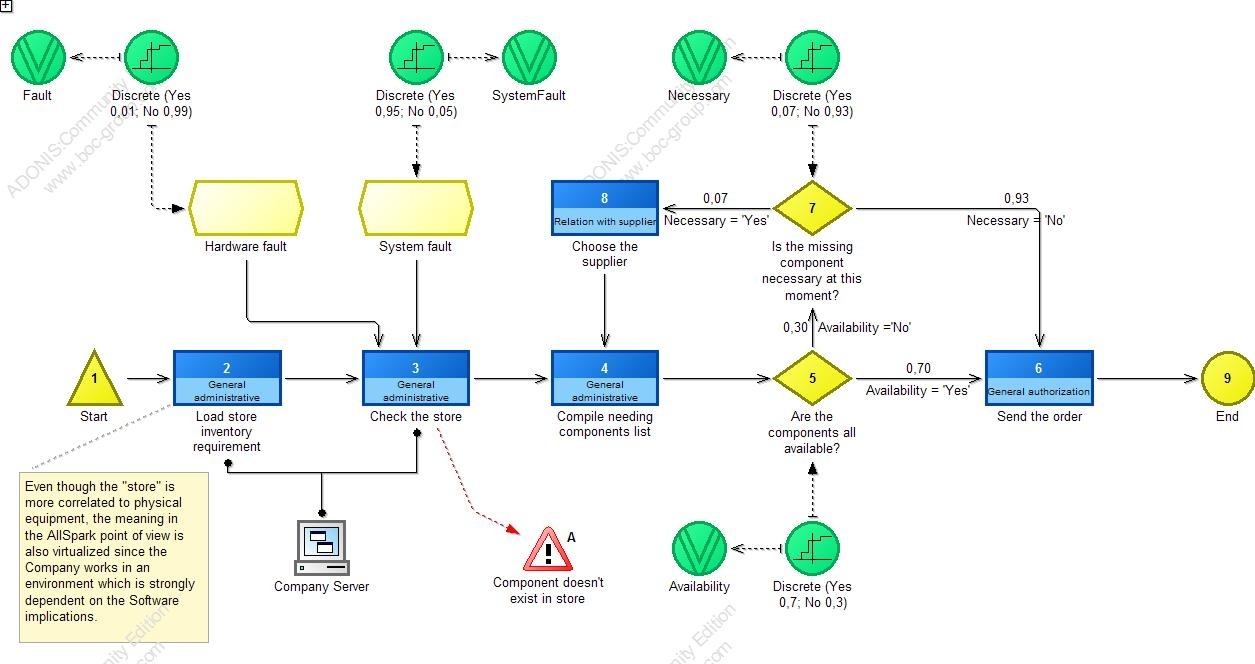
\includegraphics[scale=0.50, angle=90]{assign2/adonis/imgs/supply_man.jpg}
\caption{AllSpark Supply Management.}
\label{2img:supply_man}
\end{centering}
\end{figure}


\subsubsection{Path Analysis}
The analysis of possible path in this process shows five distinct elements, two of them with relevant probability. The most significative is the one with the 72,10\% of probability to happen and shows the favorite and expected actions with the needed components immediately available.

\begin{alltt}
Probability:   72,1000%
Execution time:  00:000:00:25:40
Waiting time:  00:000:00:00:50
Resting time:  00:000:00:00:20
Transport time:  00:000:00:00:00
Cycle time:  00:000:00:26:50
Costs:  2,000000

Supply Management 0.3 (Business process model)
========================================
Process start: Start
Activity: Load store inventory requirement
Activity: Check the store
Activity: Compile needing components list
Decision: Are the components all available? --> Availability = 'Yes'
Activity: Send the order
End: End
\end{alltt}


\subsubsection{Capacity Analysis}
This process is pretty simple and the variation from expected timing and costs are really small and the capacity analysis is according to the forseen result. By the way this process doesn't take account of the actual ending time that is the moment the order arrives at the AllSpark, but this is very diffult to model since is high dependent on the elements which the Company is looking for and an average would being be quite irrealistic.

\begin{landscape}
\begin{table}
\centering
{\tiny
\begin{tabular}{|l|l|l|l|l|l|l|}
Business process&Activity&Performer&Number&Execution time&Cycle time&Costs\\
\hline
Supply Management 0.3&&&&00:000:00:26:03&00:000:00:27:14&2,030000\\
\hline
&Choose the supplier &&0,015000&00:000:00:00:09&&0,030000\\
\hline
&&Secretary &0,015000&00:000:00:00:09&&0,030000\\
\hline
&Send the order &&1,000000&00:000:00:00:10&&0,000000\\
\hline
&&CEO &1,000000&00:000:00:00:10&&0,000000\\
\hline
&Compile needing components list &&1,015000&00:000:00:15:14&&0,000000\\
\hline
&&Secretary &1,015000&00:000:00:15:14&&0,000000\\
\hline
&Check the store &&1,000000&00:000:00:10:00&&2,000000\\
\hline
&&Secretary &1,000000&00:000:00:10:00&&2,000000\\
\hline
&Load store inventory requirement &&1,000000&00:000:00:00:30&&0,000000\\
\hline
&&Secretary &1,000000&00:000:00:00:30&&0,000000\\
\hline
Total&&&&00:000:00:26:03&&2,030000
\end{tabular}
}
\caption{Capacity analysis for Supply Management.}
\end{table}
\end{landscape}
%

%

\subsection{Human Resource Management}
The Human Resource Management business process aim to lead the main resource of the Company, that is the personnel. A good management of this resource facilitates the internal relations, improves the Company renown and image, reduce the stress factor and improve the productivity. There are several activities illustrates in figure \ref{2img:human_resources}, that combine to achieve the target. In first analysis is possibile to see that a lot of human relations are considered in this model, while the others more standard are relegated to subprocesses not shown here. The motivation is the peculiar orientation to the monitoring of variable factor that cannot be defined apriori.

A significantly number of activities are supervised by the Project Manager that is the role which best fit with the topic of the process since it is across several kind of competences and its culture is better flexible to the themes proposed, even though an official professional figure may be important here.

\begin{figure}[ht!]
\begin{centering}
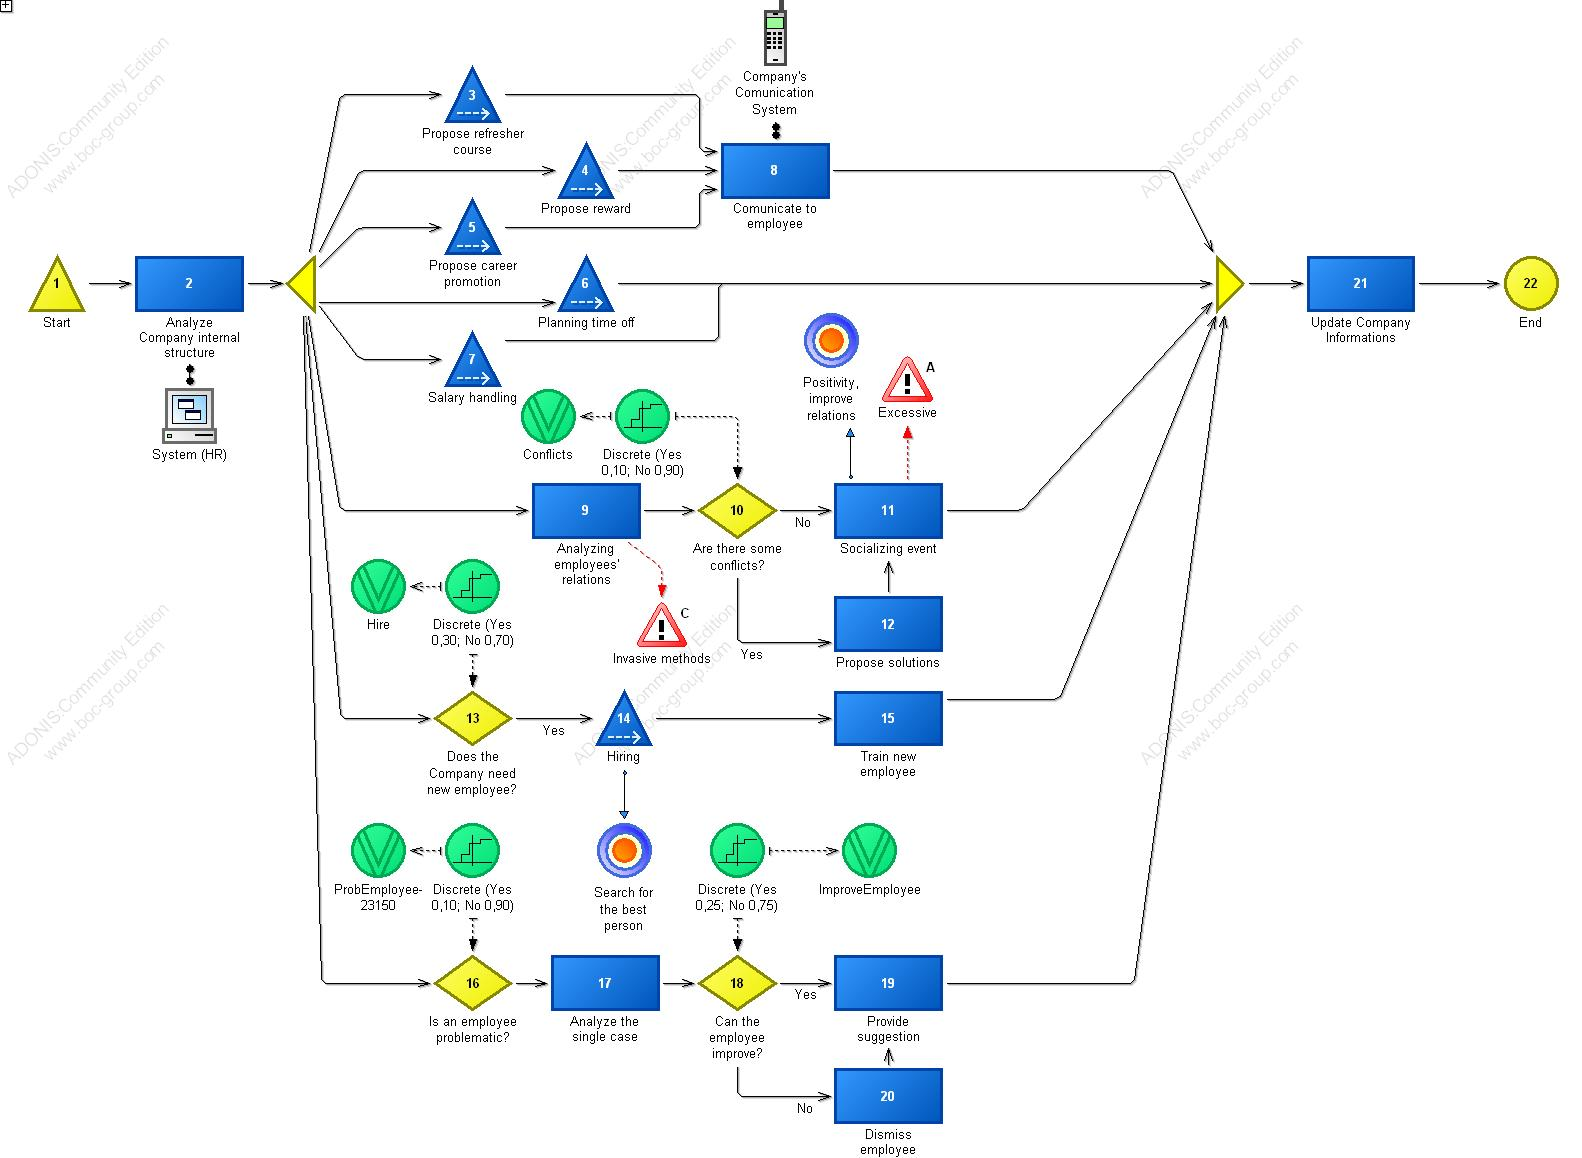
\includegraphics[scale=0.35, angle=90]{assign2/adonis/imgs/human_resources.jpg}
\caption{AllSpark Human Resources Management.}
\label{2img:human_resources}
\end{centering}
\end{figure}


\subsubsection{Path Analysis}
The path analysis results ten different paths, but only two of them are significative and are reported in the following table. Particular interesting the two paths shown differs significatively both in times and the costs even though this one is similar to the other. The two paths are completely shown straight forward the table.

The main difference is the hiring activity that requires a lot of resources to perform the task since a new element should be trained for, specially if is a young man with few experience.

Since all the activities are human's measured, is quite normal to have these results.

\begin{table}
\centering
\begin{tabular}{|l|l|l|l|l|}
Path&Probability&Execution time&Cycle time&Costs\\
\hline
1&0,5850&00:000:08:40:00&00:000:07:36:00&2060,65\\
\hline
2&0,2430&00:016:03:40:00&00:000:21:25:00&3075,65
\end{tabular}
\end{table}

\begin{alltt}
Probability:   58,5000%
Execution time:  00:000:08:40:00
Waiting time:  00:000:00:28:00
Resting time:  00:000:01:15:00
Transport time:  00:000:02:03:00
Cycle time:  00:000:07:36:00
Costs:  2060,650000

Human Resource Management 0.1 (Business process model)
========================================
Process start: Start
Activity: Analyze Company internal structure
Parallelity: Parallelity-23097
    *
    Activity: Analyzing employees' relations
    Decision: Are there some conflicts? --> Conflicts='No'
    Activity: Socializing event
    *
    Decision: Does the Company need new employee? --> Hire = 'No'
    *
    Decision: Is an employee problematic? --> Problematic='No'
    *
    Subprocess: Salary handling
    *
    Subprocess: Planning time off
    *
    Subprocess: Propose refresher course
    Activity: Comunicate to employee
    *
    Subprocess: Propose career promotion
    Activity: Comunicate to employee
    *
    Subprocess: Propose reward
    Activity: Comunicate to employee
Merging: Merging-23184
Activity: Update Company Informations
End: End

Human Resource Management 0.1 (Business process model) --> Salary handling 1 (Business process model)
========================================
Process start: Start
Activity: Salary handling
End: End

Human Resource Management 0.1 (Business process model) --> Planning time off 1 (Business process model)
========================================
Process start: Start
Activity: Planning time off
End: End

Human Resource Management 0.1 (Business process model) --> Propose refresher course 1 (Business process model)
========================================
Process start: Start
Activity: Refresh course
End: End

Human Resource Management 0.1 (Business process model) --> Propose career promotion 1 (Business process model)
========================================
Process start: Start
Activity: Career promotion
End: End

Human Resource Management 0.1 (Business process model) --> Propose reward 1 (Business process model)
========================================
Process start: Start
Activity: Reward
End: End
\end{alltt}

\begin{alltt}
Probability:   24,3000%
Execution time:  00:016:03:40:00
Waiting time:  00:002:00:38:00
Resting time:  00:003:02:15:00
Transport time:  00:001:02:03:00
Cycle time:  00:021:06:25:00
Costs:  3075,650000

Human Resource Management 0.1 (Business process model)
========================================
Process start: Start
Activity: Analyze Company internal structure
Parallelity: Parallelity-23097
    *
    Activity: Analyzing employees' relations
    Decision: Are there some conflicts? --> Conflicts='No'
    Activity: Socializing event
    *
    Decision: Does the Company need new employee? --> Hire='Yes'
    Subprocess: Hiring
    Activity: Train new employee
    *
    Decision: Is an employee problematic? --> Problematic='No'
    *
    Subprocess: Salary handling
    *
    Subprocess: Planning time off
    *
    Subprocess: Propose refresher course
    Activity: Comunicate to employee
    *
    Subprocess: Propose career promotion
    Activity: Comunicate to employee
    *
    Subprocess: Propose reward
    Activity: Comunicate to employee
Merging: Merging-23184
Activity: Update Company Informations
End: End

Human Resource Management 0.1 (Business process model) --> Salary handling 1 (Business process model)
========================================
Process start: Start
Activity: Salary handling
End: End

Human Resource Management 0.1 (Business process model) --> Planning time off 1 (Business process model)
========================================
Process start: Start
Activity: Planning time off
End: End

Human Resource Management 0.1 (Business process model) --> Propose refresher course 1 (Business process model)
========================================
Process start: Start
Activity: Refresh course
End: End

Human Resource Management 0.1 (Business process model) --> Propose career promotion 1 (Business process model)
========================================
Process start: Start
Activity: Career promotion
End: End

Human Resource Management 0.1 (Business process model) --> Propose reward 1 (Business process model)
========================================
Process start: Start
Activity: Reward
End: End

Human Resource Management 0.1 (Business process model) --> Hiring 1 (Business process model)
========================================
Process start: Start
Activity: Hiring
End: End
\end{alltt}


\subsubsection{Capacity Analysis}
In capacity analysis figure a sensible difference between the execution time and the cycle time consisting in about two days. A great contribute for the execution time is given with the hiring functions which is executed for a total of 0,30 times, but contribute significatively on the execution time. The costs are interesting particular the reward that is fixed as the attribute number indicates. Also socializing event is predetermined and this reflect the interesting of AllSpark to improve the internal relations.


\begin{landscape}
\begin{table}
\centering
{\tiny
\begin{tabular}{|l|l|l|l|l|l|l|}
Business process&Activity&Performer&Number&Execution time&Cycle time&Costs\\
\hline
Human Resource Management 0.1&&&&00:005:06:06:13&00:007:01:17:21&2372,965800\\
\hline
&Analyze Company internal structure &&1,000000&00:000:00:00:00&&0,000000\\
\hline
&&Secretary &1,000000&00:000:00:00:00&&0,000000\\
\hline
&Analyzing employees' relations &&1,000000&00:000:00:30:00&&0,300000\\
\hline
&&Area Manager &1,000000&00:000:00:30:00&&0,300000\\
\hline
&Propose solutions &&0,097000&00:000:00:05:49&&1,940000\\
\hline
&&Area Manager &0,097000&00:000:00:05:49&&1,940000\\
\hline
&Analyze the single case &&0,077000&00:000:00:02:19&&0,770000\\
\hline
&&Area Manager &0,077000&00:000:00:02:19&&0,770000\\
\hline
&Provide suggestion &&0,077000&00:000:00:00:46&&0,030800\\
\hline
&&Area Manager &0,077000&00:000:00:00:46&&0,030800\\
\hline
&Dismiss employee &&0,054000&00:000:00:00:49&&0,000000\\
\hline
&&CEO &0,054000&00:000:00:00:49&&0,000000\\
\hline
&Socializing event &&1,000000&00:000:01:00:00&&200,000000\\
\hline
&&CEO &1,000000&00:000:01:00:00&&200,000000\\
\hline
&Update Company Informations &&1,000000&00:000:00:10:00&&0,200000\\
\hline
&&Secretary &1,000000&00:000:00:10:00&&0,200000\\
\hline
&Comunicate to employee &&3,000000&00:000:00:30:00&&0,150000\\
\hline
&&Secretary &3,000000&00:000:00:30:00&&0,150000\\
\hline
&Train new employee &&0,305000&00:000:01:31:30&&4,575000\\
\hline
&&Area Manager &0,305000&00:000:01:31:30&&4,575000\\
\hline
&Refresh course &&1,000000&00:000:04:00:00&&200,000000\\
\hline
&&Area Manager &1,000000&00:000:04:00:00&&200,000000\\
\hline
&Reward &&1,000000&00:000:00:30:00&&1500,000000\\
\hline
&&CEO &1,000000&00:000:00:30:00&&1500,000000\\
\hline
&Career promotion &&1,000000&00:000:00:30:00&&100,000000\\
\hline
&&CEO &1,000000&00:000:00:30:00&&100,000000\\
\hline
&Planning time off &&1,000000&00:000:01:00:00&&10,000000\\
\hline
&&Area Manager &1,000000&00:000:01:00:00&&10,000000\\
\hline
&Salary handling &&1,000000&00:000:00:30:00&&50,000000\\
\hline
&&CEO &1,000000&00:000:00:30:00&&50,000000\\
\hline
&Hiring &&0,305000&00:004:05:45:00&&305,000000\\
\hline
&&CEO &0,305000&00:004:05:45:00&&305,000000\\
\hline
Total&&&&00:005:06:06:13&&2372,965800
\end{tabular}
}
\caption{Capacity analysis for Supply Management.}
\end{table}
\end{landscape}
%

%

\subsection{Updating Management}
This Updating Management business process is derived by the macro business process ``Systems Management'' that provides, as the name suggests, the service of ``up to date'' systems meaning softwares, both products and tools, and hardwares in order to minimize the presence of bugs, improve the efficiency and acquire new features.

The main responsible of this business process is the System Manager who has the very important role of manage all the tasks reducing the possible side effects. For certain task the System Manager is not required to be responsible since are not warning activities. The whole process is shown in figure \ref{2img:updating}.

\begin{figure}[ht!]
\begin{centering}
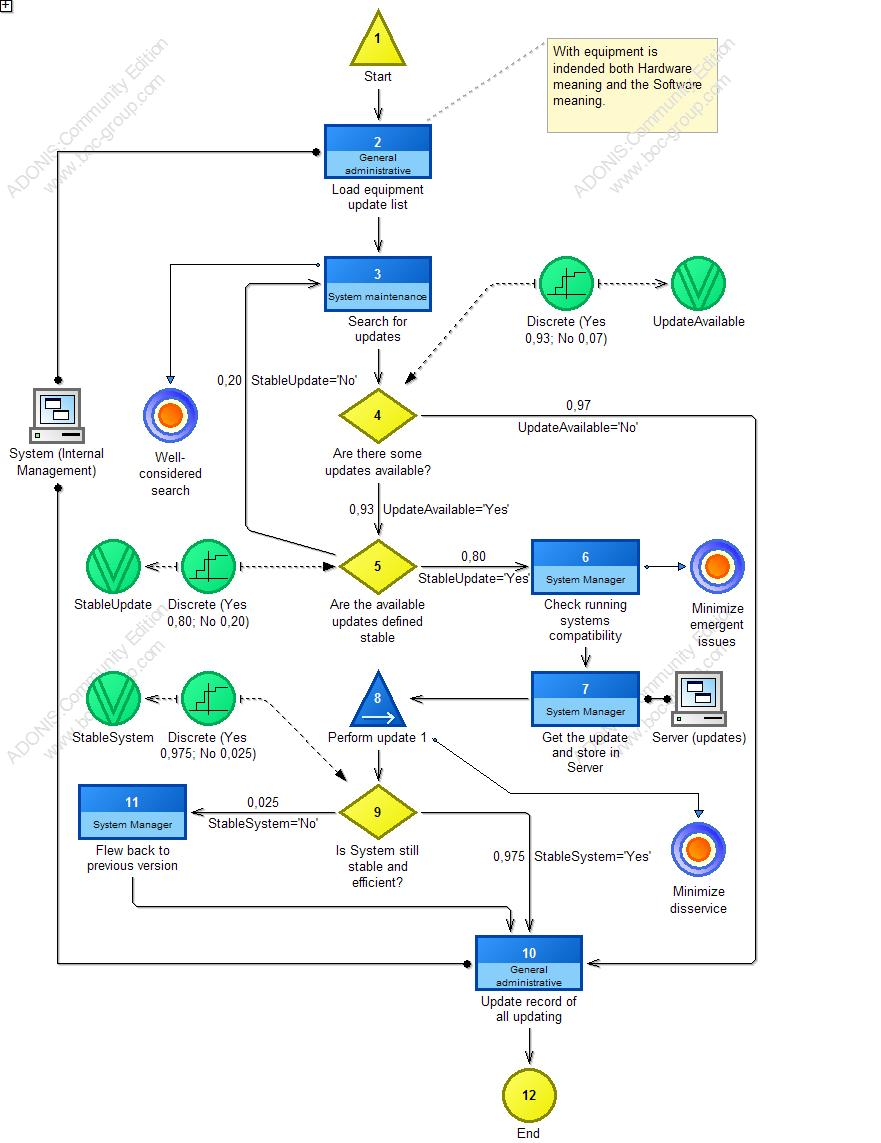
\includegraphics[scale=0.50]{assign2/adonis/imgs/updating.jpg}
\caption{AllSpark Updating Management.}
\label{2img:updating}
\end{centering}
\end{figure}


\subsubsection{Path Analysis}
According to the results of path analysis, an update is expected to succeed with the probability of 73,70\% as foreseen. The whole process is quite cheaper and the time is considered with nothing going badly. The following report returns the complete information about it.

\begin{alltt}
Probability:   73,7000\%
Execution time:  00:000:01:21:00
Waiting time:  00:000:00:02:00
Resting time:  00:000:00:12:00
Transport time:  00:000:00:10:00
Cycle time:  00:000:01:45:00
Costs:  1,980000

Updating Management 0.3 (Business process model)
========================================
Process start: Start
Activity: Load equipment update list
Activity: Search for updates
Decision: Are there some updates available? --> UpdateAvailable='Yes'
Decision: Are the available updates defined stable --> StableUpdate='Yes'
Activity: Check running systems compatibility
Activity: Get the update and store in Server
Subprocess: Perform update
Decision: Is System still stable and efficient? --> StableSystem='Yes'
Activity: Update record of all updating
End: End

Updating Management 0.3 (Business process model) --> Perform update 1 (Business process model)
========================================
Process start: Start
Activity: Perform update
End: End
\end{alltt}


\subsubsection{Capacity Analysis}
The capacity analysis for this process shows the interesting activites' report which are strongly dependent by the System Manager which is represented by either Sysadmin or Area Manager distinguishing the cases in which he is the real responsible of the entire AllSpark's system structure.

\begin{landscape}
\begin{table}
\centering
{\tiny
\begin{tabular}{|l|l|l|l|l|l|l|}
Business process&Activity&Performer&Number&Execution time&Cycle time&Costs\\
\hline
Updating Management 0.3&&&&00:000:01:23:33&00:000:01:48:07&5,966800\\
\hline
&Load equipment update list &&1,000000&00:000:00:01:00&&0,200000\\
\hline
&&Secretary &1,000000&00:000:00:01:00&&0,200000\\
\hline
&Update record of all updating &&1,000000&00:000:00:15:00&&0,900000\\
\hline
&&Secretary &1,000000&00:000:00:15:00&&0,900000\\
\hline
&Search for updates &&1,240000&00:000:00:24:48&&0,248000\\
\hline
&&Sysadmin &1,240000&00:000:00:24:48&&0,248000\\
\hline
&Check running systems compatibility &&0,910000&00:000:00:09:06&&0,273000\\
\hline
&&Area Manager &0,910000&00:000:00:09:06&&0,273000\\
\hline
&Flew back to previous version &&0,020000&00:000:00:01:48&&4,000000\\
\hline
&&Area Manager &0,020000&00:000:00:01:48&&4,000000\\
\hline
&Get the update and store in Server &&0,910000&00:000:00:13:39&&0,273000\\
\hline
&&Area Manager &0,910000&00:000:00:13:39&&0,273000\\
\hline
&Perform update &&0,910000&00:000:00:18:12&&0,072800\\
\hline
&&Sysadmin &0,910000&00:000:00:18:12&&0,072800\\
\hline
Total&&&&00:000:01:23:33&&5,966800
\end{tabular}
}
\caption{Capacity analysis for Updating Management.}
\end{table}
\end{landscape}
%

%

\subsection{Documentation repository}
The ``Documentation repository'' is another business process that is not directly connected to productivity or to the Company's lifecycle, but is needed to clearify the products in order to give to client a professional description, but also to facilitate future works based upon it. Particulary the process aim to draw up both commeting information on the project's files and the separated official documentation (that is both the documentation project and the documentation of use).

The main responsible of the task is the Analyst that supervise all the main activities. Also important are the role of Developer (who may be also a sysadmin if the topic is inherent the Systems) and Secretary who direct works on the documentation's building.

\begin{figure}[ht!]
\begin{centering}
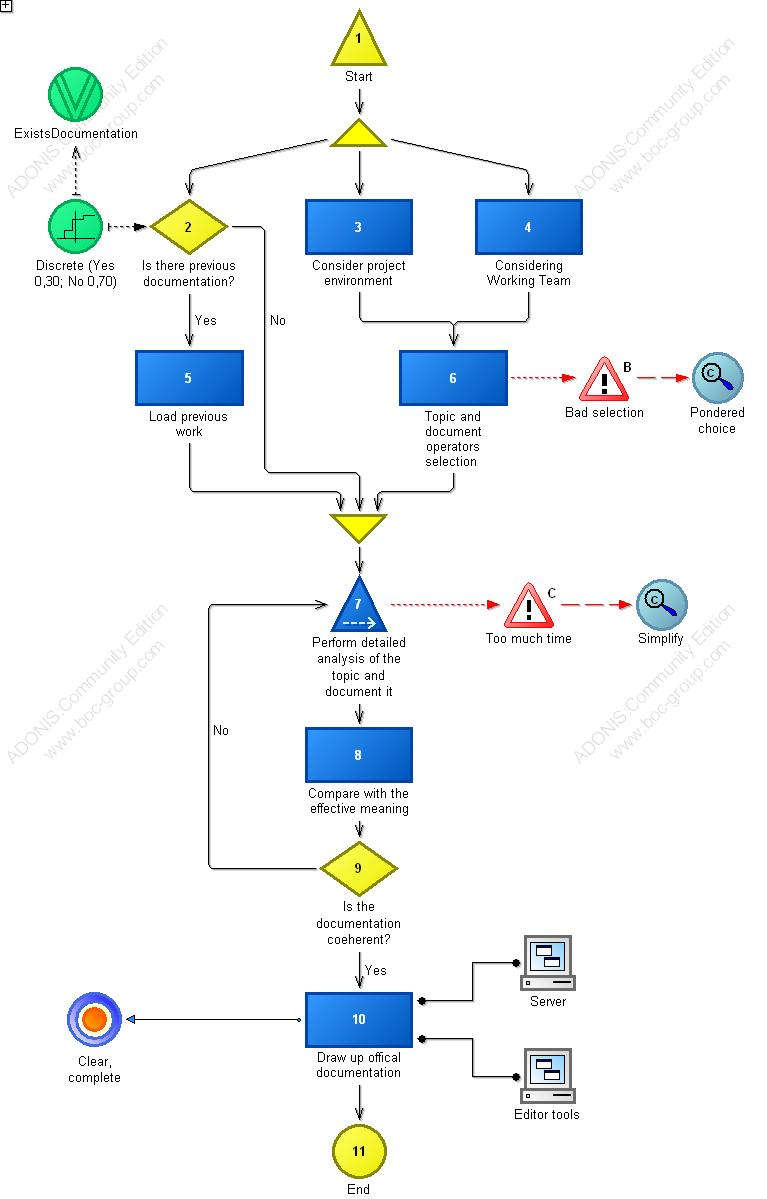
\includegraphics[scale=0.50]{assign2/adonis/imgs/documentation.jpg}
\caption{AllSpark Documentation repository.}
\label{2img:documentation}
\end{centering}
\end{figure}


\subsubsection{Path Analysis}
The path analysis return seven possible paths. Only two of them are interesting in terms of probability, but they are quite identical so only the most probability will be shown. The time is very low for a documentation and this is strange, but is important to underline that the process was modeled bearing that a project have at least a person, but may be different; this time is about the one person work and so the entire business process should be calibrate for each possible project which involve different people.

\begin{alltt}
Probability:   60,3000\%
Execution time:  00:000:03:20:00
Waiting time:  00:000:00:01:00
Resting time:  00:000:00:50:00
Transport time:  00:000:00:00:00
Cycle time:  00:000:03:16:00
Costs:  4,300000

Documentation repository 0.1 (Business process model)
========================================
Process start: Start
Parallelity: Parallelity-22082
    *
    Activity: Consider project environment
    Activity: Topic and document operators selection 
    *
    Activity: Considering Working Team
    Activity: Topic and document operators selection 
    *
    Decision: Is there previous documentation? --> ExistsDocumentation='No'
Merging: Merging-22112
Subprocess: Perform detailed analysis of the topic and document it
Activity: Compare with the effective meaning
Decision: Is the documentation coeherent? --> DocumentCoherency='Yes'
Activity: Draw up offical documentation
End: End

Documentation repository 0.1 (Business process model) --> Document 1 (Business process model)
========================================
Process start: Start
Activity: Documentation
End: End
\end{alltt}


\subsubsection{Capacity Analysis}
The capacity analysis of this process permits to observe the difference between execution time and cycle time which is possible thanking the parallelism which permits to reduce the global timing.

\begin{landscape}
\begin{table}
\centering
{\tiny
\begin{tabular}{|l|l|l|l|l|l|l|}
Business process&Activity&Performer&Number&Execution time&Cycle time&Costs\\
\hline
Documentation repository 0.1&&&&00:000:03:51:20&00:000:03:34:20&4,614100\\
\hline
&Load previous work &&0,283000&00:000:00:14:09&&0,084900\\
\hline
&&Secretary &0,283000&00:000:00:14:09&&0,084900\\
\hline
&Consider project environment &&1,000000&00:000:00:20:00&&0,400000\\
\hline
&&Analyst &1,000000&00:000:00:20:00&&0,400000\\
\hline
&Considering Working Team &&1,000000&00:000:00:20:00&&0,400000\\
\hline
&&Area Manager &1,000000&00:000:00:20:00&&0,400000\\
\hline
&Draw up offical documentation &&1,000000&00:000:00:30:00&&1,500000\\
\hline
&&Programmer &1,000000&00:000:00:30:00&&1,500000\\
\hline
&Topic and document operators selection  &&2,000000&00:000:00:40:00&&0,800000\\
\hline
&&Analyst &2,000000&00:000:00:40:00&&0,800000\\
\hline
&Compare with the effective meaning &&1,191000&00:000:00:23:49&&0,476400\\
\hline
&&Analyst &1,191000&00:000:00:23:49&&0,476400\\
\hline
&Documentation &&1,191000&00:000:01:23:22&&0,952800\\
\hline
&&Programmer &1,191000&00:000:01:23:22&&0,952800\\
\hline
Total&&&&00:000:03:51:20&&4,614100
\end{tabular}
}
\caption{Capacity analysis for Document repository.}
\end{table}
\end{landscape}
%

%